\documentclass[border=3pt]{standalone}
\usepackage[T1]{fontenc}\usepackage{lmodern}\usepackage{amsmath}
\usepackage{tikz}
\usetikzlibrary{patterns,arrows.meta,calc}
\definecolor{ink}{HTML}{1B1F3B}\definecolor{acc}{HTML}{4B3FA8}\definecolor{org}{HTML}{E08A1E}\definecolor{red}{HTML}{C0392B}
\begin{document}
\normalsize
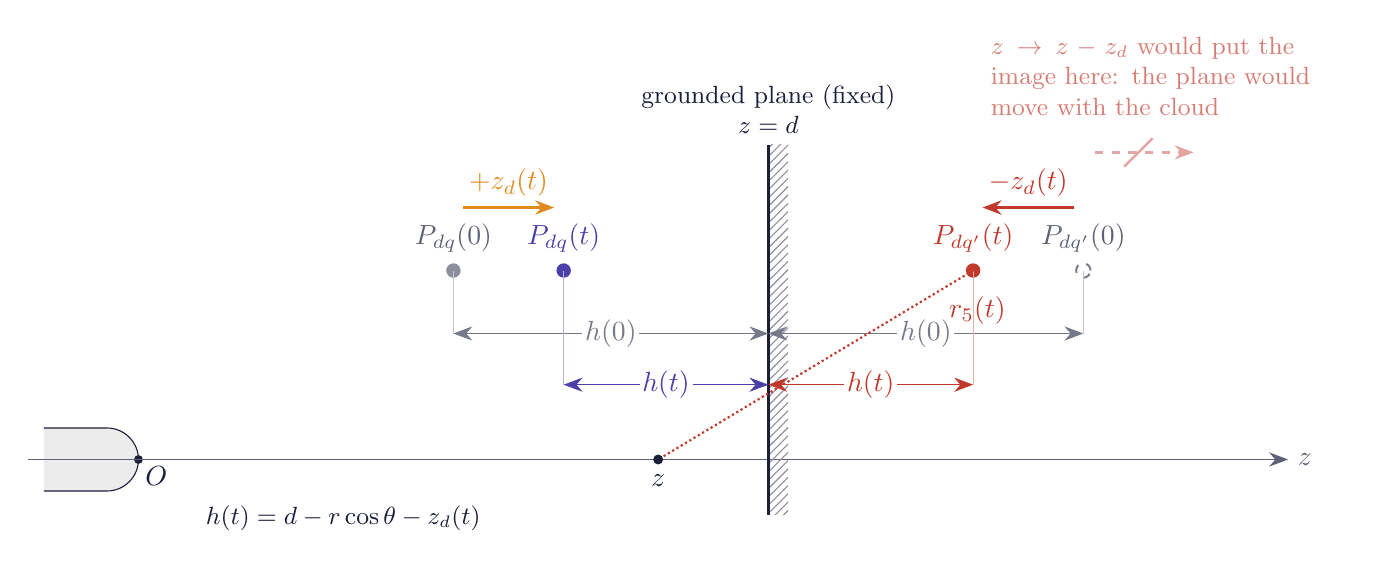
\begin{tikzpicture}[>={Stealth[length=2.4mm]}]
\filldraw[fill=gray!15, draw=ink] (-1.2,0.4) -- (-0.4,0.4) arc[start angle=90, end angle=-90, radius=0.4] -- (-1.2,-0.4);
\fill[ink] (0,0) circle (1.6pt) node[below right=-1pt] {$O$};
\draw[->, ink!70] (-1.4,0) -- (14.6,0) node[right] {$z$};
\fill[pattern=north east lines, pattern color=ink!50] (8.0,-0.7) rectangle (8.25,4.0);
\draw[ink, line width=1pt] (8.0,-0.7) -- (8.0,4.0) node[above, align=center, font=\small] {grounded plane (fixed)\\$z=d$};
\fill[ink!50] (4.0,2.4) circle (2.6pt) node[above=3pt, ink!70] {$P_{dq}(0)$};
\fill[acc] (5.4,2.4) circle (2.6pt) node[above=3pt] {$P_{dq}(t)$};
\draw[->, org, line width=1.1pt] (4.12,3.2) -- (5.28,3.2) node[midway, above] {$+z_{d}(t)$};
\fill[white] (12.0,2.4) circle (2.6pt); \draw[ink!60, dashed, line width=0.7pt] (12.0,2.4) circle (2.6pt);
\node[ink!70, above=3pt] at (12.0,2.4) {$P_{dq'}(0)$};
\fill[red] (10.6,2.4) circle (2.6pt) node[above=3pt] {$P_{dq'}(t)$};
\draw[->, red, line width=1.1pt] (11.88,3.2) -- (10.719999999999999,3.2) node[midway, above] {$-z_{d}(t)$};
\draw[<->, ink!60] (4.0,1.6) -- (8.0,1.6) node[midway, fill=white, inner sep=1pt] {$h(0)$};
\draw[<->, ink!60] (8.0,1.6) -- (12.0,1.6) node[midway, fill=white, inner sep=1pt] {$h(0)$};
\draw[<->, acc] (5.4,0.95) -- (8.0,0.95) node[midway, fill=white, inner sep=1pt] {$h(t)$};
\draw[<->, red] (8.0,0.95) -- (10.6,0.95) node[midway, fill=white, inner sep=1pt] {$h(t)$};
\draw[ink!25] (4.0,2.4) -- (4.0,1.6); \draw[ink!25] (12.0,2.4) -- (12.0,1.6);
\draw[acc!40] (5.4,2.4) -- (5.4,0.95); \draw[red!40] (10.6,2.4) -- (10.6,0.95);
\draw[->, red!45, dashed, line width=0.8pt] (12.15,3.9) -- (13.4,3.9);
\draw[red!45, line width=0.9pt] (12.52,3.7199999999999998) -- (12.879999999999999,4.08);
\node[red!65, font=\small, align=left, anchor=south west, text width=4.4cm] at (10.7,4.25) {$z\to z-z_{d}$ would put the image here: the plane would move with the cloud};
\draw[red, densely dotted, line width=0.8pt] (10.6,2.4) -- (6.6,0) node[pos=0.1, below right=-1pt] {$r_{5}(t)$};
\fill[ink] (6.6,0) circle (1.8pt) node[below=2pt] {$z$};
\node[ink, font=\small] at (2.6,-0.75) {$h(t)=d-r\cos\theta-z_{d}(t)$};
\end{tikzpicture}
\end{document}
